\chapter{操纵路径的命令}
构建路径后,可以对路径进行多种操纵以改变路径的呈现形态。一般常用的命令以以下这些:

\noindent
\begin{ditemize}
	\forcsvlist{\tcbitem}{draw, fill, filldraw, pattern, shade, shadedraw, clip, useasboundingbox}

\end{ditemize}

\section{颜色color}
可以用\texinline{\colorlet}命令来定义新的颜色,\texinline{black!50}会产生中灰色\tikz\filldraw[black!50] circle (5pt);
。这样的颜色取值模式很方便,并且可以与其他颜色继续混合。

\section{绘制draw}
\texinline{\draw}命令用来绘制路径,除了路径的颜色以外,还有一些其他的属性会影响整个图形的外观。
\subsection{线条粗细、端头、接头}
\texinline{line width}属性有以下一些预设值:
\begin{ditemize}
	\forcsvlist{\tcbitem}{ultra thin 0.1pt, very thin 0.2pt,thin 0.4pt, semithick 0.6pt, thick 0.8pt, very thick 1.2pt, ultra thick 1.6pt}
\end{ditemize}
\texinline{line cap}有三种样式\forcsvlist{\texinline}{round, butt, rect}。
\begin{texlst}
	
\begin{tikzpicture}
		\begin{scope}[line width=10pt]
			\draw[line cap=round] (0,1) -- +(1,0);
			\draw[line cap=butt] (0,.5) -- +(1,0);
			\draw[line cap=rect] (0,0) -- +(1,0);
		\end{scope}
		\draw[white, line width=2pt] (0,0) -- +(1,0) (0,.5) -- +(1,0) (0,1) -- +(1,0);
	\end{tikzpicture}
\end{texlst}

转角处的连接也有三种样式\forcsvlist{\texinline}{round, bevel, miter}
\begin{texlst}
	
\begin{tikzpicture}[line width=10pt]
		\draw[line join=round] (0,0) -- ++(.5,1) -- ++(.5,-1);
		\draw[line join=bevel] (1.25,0) -- ++(.5,1) -- ++(.5,-1);
		\draw[line join=miter] (2.5,0) -- ++(.5,1) -- ++(.5,-1);
		\useasboundingbox(0,1.5);
	\end{tikzpicture}
\end{texlst}

\texinline{miter}尖角模式下,如果夹角太小,会导致尖头太长,这里可以通过设置\texinline{miter
	limit},如果尖头的长度超过线宽的\texinline{miter limit}倍就自动转换成平头的,默认值是10。
\begin{texlst}
	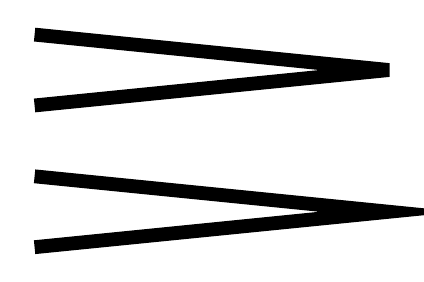
\begin{tikzpicture}[line width=5pt, scale=0.9]
		\draw (0,0) -- ++(5,.5) -- ++(-5, .5);
		\draw[miter limit=25] (0,-2) -- ++(5,.5) -- ++(-5, .5);
	\end{tikzpicture}
\end{texlst}

\subsection{点划线模式 dash pattern}
\begin{texlst}
	\begin{tikzpicture}[dash pattern=on 2pt off 3pt on 4pt off 4pt]
		\draw (0,0) -- (3.5cm, 0);
	\end{tikzpicture}
\end{texlst}

此外还可以通过\texinline{dash phase}来错开。
\begin{texlst}
	\begin{tikzpicture}[dash pattern=on 20pt off 10pt]
		\draw[dash phase=0pt] (0pt, 3pt) -- (3.5cm, 3pt);
		\draw[dash phase=10pt] (0pt, 0pt) -- (3.5cm, 0pt);
	\end{tikzpicture}
\end{texlst}

还可以将\texinline{dash pattern}与\texinline{dash phase}写到一起。
\begin{texlst}
	\begin{tikzpicture}
		\draw[dash=on 20pt off 10pt phase 0pt] (0pt,3pt) -- (3.5cm, 3pt);
		\draw[dash=on 20pt off 10pt phase 10pt] (0pt,0pt) -- (3.5cm, 0pt);
	\end{tikzpicture}
\end{texlst}
注意,这里\texinline{pattern}给省略了。

其他的所有线的样式其实都可以从\texinline{dash pattern}里面变化而来,比如实线(solid)就是\\
\texinline{on 1pt off 0pt},等等。\tikzname 提供了一些预设好的样式:
\begin{ditemize}
	\forcsvlist{\tcbitem}{solid, dotted, densly dotted, loosely dotted, dashed, loosely dash, densly dashed, dash dot,
		densely dash dot, loosely dash dot, dash dot dot, densely dash dot dot, loosely dash dot dot}
\end{ditemize}

\subsection{双线 double}
双线的中间默认是白色的,初始线距0.6pt。
\begin{texlst}
	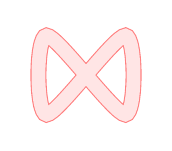
\begin{tikzpicture}
		\draw[double=red!10, red!50, double distance=5pt] plot[smooth cycle] coordinates{(0,0) (1,1) (1,0) (0,1)};
	\end{tikzpicture}
\end{texlst}
此外,线距还有两个变种,线中心距\texinline{double distance between line center}和等号中心距\\\texinline{double equal sign
	distance}。

\section{箭头 arrow tips}
普通的箭头经常使用,其他的箭头样式后面再看。

\section{填充 fill}
填充颜色只需要给\texinline{fill}选项指定一个颜色就行。此外,\tikzname 还提供了一些预设的图案\texinline{pattern},
需要加载\texinline{patterns}库。
\begin{texlst}
	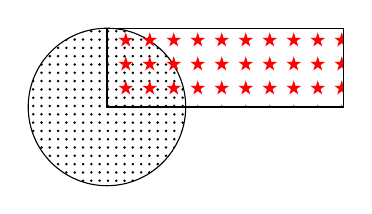
\begin{tikzpicture}
		\draw[pattern=dots] (0,0) circle (1cm);
		\draw[pattern=fivepointed stars, pattern color=red] (0,0) rectangle (3,1);
	\end{tikzpicture}
\end{texlst}

填充模式默认为\texinline{nonzero rule},就是全部填充。另外一种叫\texinline{even odd
	rule}也就是根据虚拟的一条线穿过路径是偶数的情况下认为是在外部,奇数为内部。

\begin{texlst}
	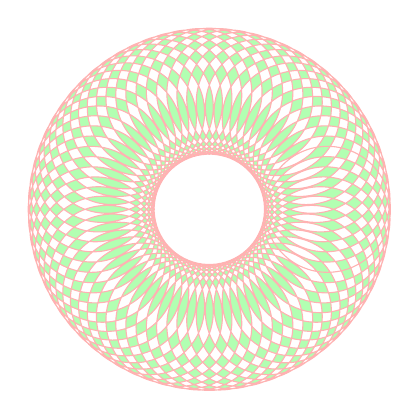
\begin{tikzpicture}
		\draw[even odd rule, fill=green!30, draw=red!30]
		\foreach \a in {0, 5, ..., 360}{(\a:1.5cm) circle (.8cm)};
	\end{tikzpicture}
\end{texlst}

\section{图片填充}
先来看一个示例:
\begin{texlst}
	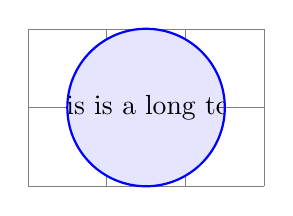
\begin{tikzpicture}
		\draw [help lines] (0,0) grid (3,2);
		\filldraw [fill=blue!10, draw=blue, thick] (1.5,1) circle (1)
		[path picture={
						\node at (path picture bounding box.center){
							This is a long text.
						};
					}];
	\end{tikzpicture}
\end{texlst}

再来一个:
\begin{texlst}
	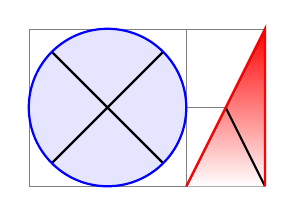
\begin{tikzpicture}[cross/.style={path picture={
							\draw[black]
							(path picture bounding box.south east) --
							(path picture bounding box.north west)
							(path picture bounding box.south west) --
							(path picture bounding box.north east);
						}}]
		\draw [help lines] (0,0) grid (3,2);
		\filldraw [cross, fill=blue!10, draw=blue, thick] (1,1) circle (1);
		\path [cross, top color=red, draw=red, thick] (2,0) -- (3,2) -- (3,0);
	\end{tikzpicture}
\end{texlst}

第二个红色的示例我目前还没有搞清楚,后来有机会再深入吧。这里当然也可以用磁盘上的图片,就不试验了。

\section{渐变 Shading}
渐变与填充相比,区别就是填充的是纯色,而渐变填充的颜色是有变化的。

\begin{texlst}
	
\begin{tikzpicture}
		\shade circle (1cm);
	\end{tikzpicture}
\end{texlst}
默认的渐变是轴向的\texinline{axis},上部的颜色是灰,下部是白。另外还有两种\forcsvlist{\texinline}{radial 辐射, ball
	球形}。

\begin{texlst}
	\begin{tikzpicture}
		\shadedraw [shading=axis, shading angle=135, lower left=blue] (0,0) rectangle (1,1);
		% 这个里面的渐变角度和指定的lower left的颜色位置是有叠加效果的。
		\shadedraw [xshift=1.5cm, shading=radial, inner color=blue!50, outer color=green!20] (0,0) rectangle (1,1);
		\shadedraw [xshift=3.5cm, shading=ball, ball color=red!60, draw=red] (0,0.5) circle(0.5cm);
	\end{tikzpicture}
\end{texlst}

其他更多的渐变用法后面会继续学到。

\section{包围盒子 bounding box}
\texinline{use as bounding box}这个功能很强大,这个让一些设置变得非常简单。
\begin{texlst}
	Left of picture
	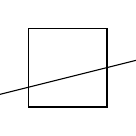
\begin{tikzpicture}
		\draw[use as bounding box] (2,0) rectangle (3,1);
		\draw (1,0) -- (4,.75);
	\end{tikzpicture}
	right of picture
\end{texlst}

另外,还有一个\texinline{current bounding box}也非常好用。
\begin{texlst}
	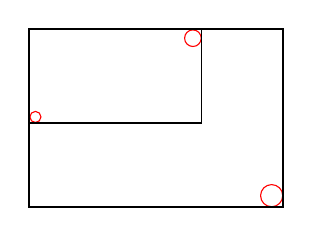
\begin{tikzpicture}
		\draw [red] (0,0) circle (2pt);
		\draw [red] (2,1) circle (3pt);

		\draw (current bounding box.south west) rectangle (current bounding box.north east);

		\draw [red] (3,-1) circle (4pt);

		\draw[thick] (current bounding box.south west) rectangle (current bounding box.north east);
	\end{tikzpicture}
\end{texlst}

\texinline{trim left}和\texinline{trim right}会将设定值的左边或者右边忽略掉。如果设定值是一个坐标的话只会使用$x$的值。

\begin{texlst}
	text before image
	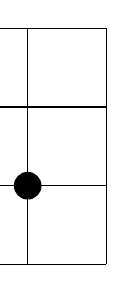
\begin{tikzpicture}[trim left] %默认值是0pt
		\draw (-1,-1) grid (1,2);
		\fill (0,0) circle (5pt);
	\end{tikzpicture}
	text after image.
\end{texlst}

\section{裁剪 Clip}
\begin{texlst}
	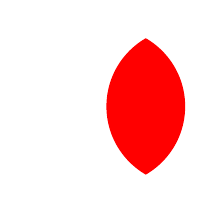
\begin{tikzpicture}
		\clip (0,0) circle (1cm);
		\fill[red] (1,0) circle (1cm);
	\end{tikzpicture}
\end{texlst}

\section{多重动作 Preaction \& Postaction}
\texinline{preaction}和\texinline{postaction}分别可以在绘制路径之前与之后进行额外的动作。
\begin{texlst}
	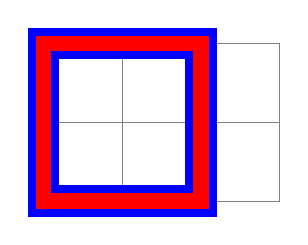
\begin{tikzpicture}
		\draw [help lines] (0,0) grid (3,2);

		\draw[preaction={draw, line width=4mm, blue}]
		[line width=2mm, red] (0,0) rectangle (2,2);
	\end{tikzpicture}
\end{texlst}

用这个还可以做一个阴影效果:
\begin{texlst}
	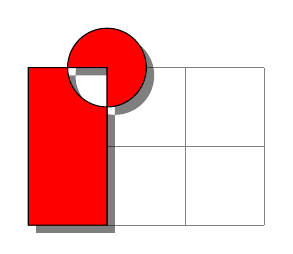
\begin{tikzpicture}
		\draw [help lines] (0,0) grid (3,2);
		\draw [preaction={fill=black, opacity=.5, transform canvas={xshift=1mm, yshift=-1mm}}]
		[fill=red] (0,0) rectangle (1,2)
		(1,2) circle (5mm);
	\end{tikzpicture}
\end{texlst}

\texinline{preaction}或者\texinline{postaction}的效果还可以叠加。
\begin{texlst}
	\usetikzlibrary{patterns}
	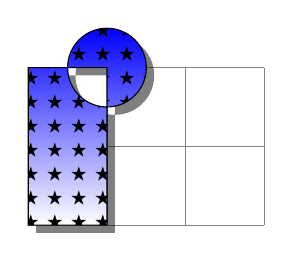
\begin{tikzpicture}
		\draw [help lines] (0,0) grid (3,2);
		\draw[pattern=fivepointed stars] [preaction={fill=black, opacity=.5, transform canvas={xshift=1mm, yshift=-1mm}}]
		[preaction={top color=blue, bottom color=white}]
		(0,0) rectangle (1,2)
		(1,2) circle (5mm);
	\end{tikzpicture}
\end{texlst}

下面是一个复杂的示例:
\begin{texlst}
	\usetikzlibrary{fadings, patterns}
	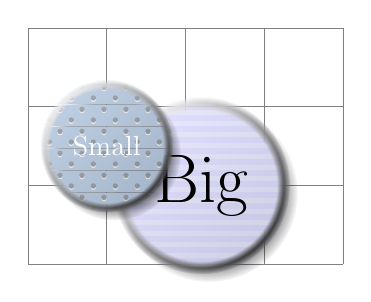
\begin{tikzpicture}
		[button/.style={
		preaction={fill=black, path fading=circle with fuzzy edge 20 percent, opacity=0.5, transform
		canvas={xshift=1mm, yshift=-1mm}},
		preaction={pattern=#1, path fading=circle with fuzzy edge 15 percent},
		preaction={top color=white,
				bottom color=black!50,
				shading angle=45,
				path fading=circle with fuzzy edge 15 percent, opacity=.2},
		preaction={path fading=fuzzy ring 15 percent,
				top color=black!5,
				bottom color=black!80,
				shading angle=45},
		inner sep=2ex
		},
		button/.default=horizontal lines light blue,
		circle
		]
		\draw [help lines] (0,0) grid (4,3);

		\node[button] at (2.2,1) {\Huge Big};
		\node[button=crosshatch dots light steel blue, text=white] at (1,1.5){Small};
	\end{tikzpicture}
\end{texlst}

这个示例对我来讲有点复杂,因为\texinline{patterns}里面的内容了解很少。以后再说。

下面再看两个\texinline{postaction}的示例:
\begin{texlst}
	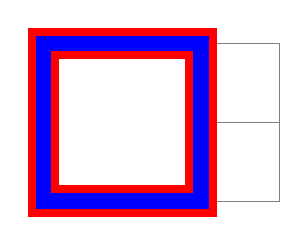
\begin{tikzpicture}
		\draw [help lines] (0,0) grid (3,2);

		\draw
		[postaction={draw, line width=2mm, blue}]
		[line width=4mm, red, fill=white] (0,0) rectangle (2,2);
	\end{tikzpicture}
\end{texlst}

\begin{texlst}
	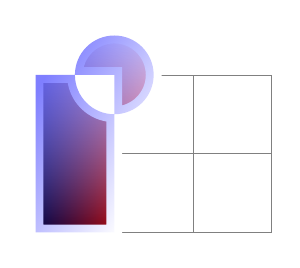
\begin{tikzpicture}
		\draw[help lines] (0,0) grid (3,2);
		\draw
		[postaction={path fading=south, fill=white}]
		[postaction={path fading=south, fading angle=45, fill=blue, opacity=.5}]
		[left color=black, right color=red, draw=white, line width=2mm]
		(0,0) rectangle (1, 2)
		(1,2) circle (5mm);
	\end{tikzpicture}
\end{texlst}

\section{装饰和变形 Decorating and Morphing}
装饰给路径添加一些内容,而变形则是改变路径的形状。

\begin{texlst}
	\usetikzlibrary{decorations.pathmorphing}
	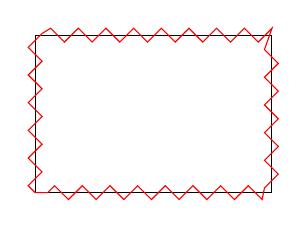
\begin{tikzpicture}
		\draw (0,0) rectangle (3,2);
		\draw [red, decorate, decoration=zigzag] (0,0) rectangle (3,2);
	\end{tikzpicture}
\end{texlst}

\begin{texlst}
	\begin{tikzpicture}
		\node [circular drop shadow={shadow scale=1.05},
			minimum size=3.13cm,
			decorate,
			decoration=zigzag,
			fill=blue!20,
			draw,
			thick,
			circle] {Hello!};
	\end{tikzpicture}
\end{texlst}

具体的内容会在后面的章节里面详细了解。
